\documentclass{article}
\usepackage{graphicx} % Required for inserting images

\usepackage{tikz}
\usetikzlibrary{automata,positioning}

\begin{document}

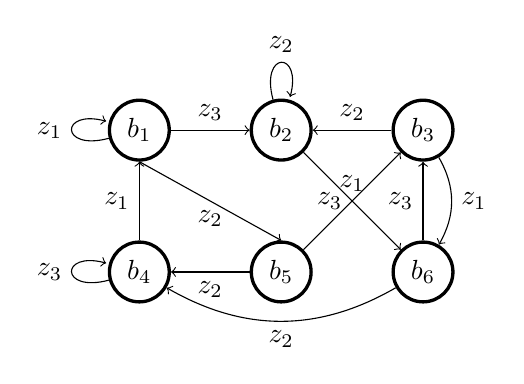
\begin{tikzpicture}[
roundnode/.style={circle, draw=black!255, fill=white!0, very thick, minimum size=7mm},
]
%Nodes
\node[roundnode]        (v1)       [] {$b_1$};
\node[roundnode]        (v2)       [right=of v1] {$b_2$};
\node[roundnode]        (v3)       [right=of v2] {$b_3$};
\node[roundnode]        (v4)       [below=of v1] {$b_4$};
\node[roundnode]        (v5)       [right=of v4] {$b_5$};
\node[roundnode]        (v6)       [right=of v5] {$b_6$};

%Lines
\path (v1) edge [loop left] node {$z_1$} (v1);
\draw[->] (v1.east) -- (v2.west) node [midway, above, sloped] (TextB1B2) {$z_3$};
\path (v2) edge [loop above] node {$z_2$} (v2);

\draw[->] (v3.west) -- (v2.east) node [midway, above, sloped] (TextB1B2) {$z_2$};

\draw[->] (v4.north) -- (v1.south) node [midway, left] (TextB1B2) {$z_1$};
\path (v4) edge [loop left] node {$z_3$} (v4);

\draw[->] (v5.west) -- (v4.east) node [midway, below] (TextB1B2) {$z_2$};

\draw[->] (v1.south) -- (v5.north) node [midway, below] (TextB1B2) {$z_2$};
\path[->] (v5) edge node [above, left] {$z_3$} (v3);

%\draw[->] (v3) to [out=20, in=20] (v6) node [midway, below,left] (TextB1B2) {t};
\path[->] (v3) edge [bend left] node [right] {$z_1$} (v6);
\path[->] (v6) edge node [left] {$z_3$} (v3);
\path[->] (v6) edge [bend left] node [below] {$z_2$} (v4);

\path[->] (v2) edge node [above] {$z_1$} (v6);

\end{tikzpicture}


\end{document}
